%!TeX root=../tese.tex
%("dica" para o editor de texto: este arquivo é parte de um documento maior)
% para saber mais: https://tex.stackexchange.com/q/78101

\chapter{Resultados da avaliação da simulação}
\label{cap_resultados}

Os resultados da avaliação da simulação se encontram divididos em duas seções. A primeira se refere ao formulário de usabilidade, no qual obtivemos 26 respostas dos alunos presentes. A segunda é referente às respostas da atividade de aprendizado, na qual tivemos 13 respostas. Em virtude do tempo limitado durante a aula, alguns dos alunos não conseguiram terminar de preencher o segundo formulário, da atividade de aprendizado, por isso, obtivemos menos respostas nele.

\section{Formulário de usabilidade}

O formulário de usabilidade adaptado do questionário SUS foi preenchido pelos alunos logo após eles terminarem de explorar a simulação. Dos 26 alunos que o responderam, 12 não haviam tido contato anterior com programação e 14 já haviam tido. Para analisar as respostas, separamos os resultados entre esses dois grupos de estudantes.

A Figura \ref{figure:likert_sim} apresenta as respostas dos alunos que haviam tido contato anterior com programação. Dentro desse grupo de alunos, a maioria respondeu que gostaria de explorar mais a simulação (85,8\%). Apenas 14,3\% ficaram confusos com a ferramenta, sendo que 64,3\% dos estudantes concordaram que ela foi fácil de usar. Ademais, 64,3\% desses alunos acreditam que não precisariam de ajuda para explorar o MVP e 21,4\% precisariam. Em consonância, 64,3\% responderam que sabiam o que era preciso fazer para usar a simulação. Também podemos observar que somente 21,4\% das crianças acharam que algumas coisas na simulação não fizeram sentido e 14,3\% delas, que tiveram que fazer algumas coisas estranhas na ferramenta. Além disso, a maioria dos usuários (78,6\%) acredita que seus amigos poderiam aprender a usar a simulação muito rápido e se sentiram confiantes enquanto a exploravam. Por fim, 28,6\% dos alunos acham que tiveram que aprender muitas coisas antes de usar o MVP, enquanto a maioria discorda (57,2\%).

\begin{figure}[h!]
    \centering
    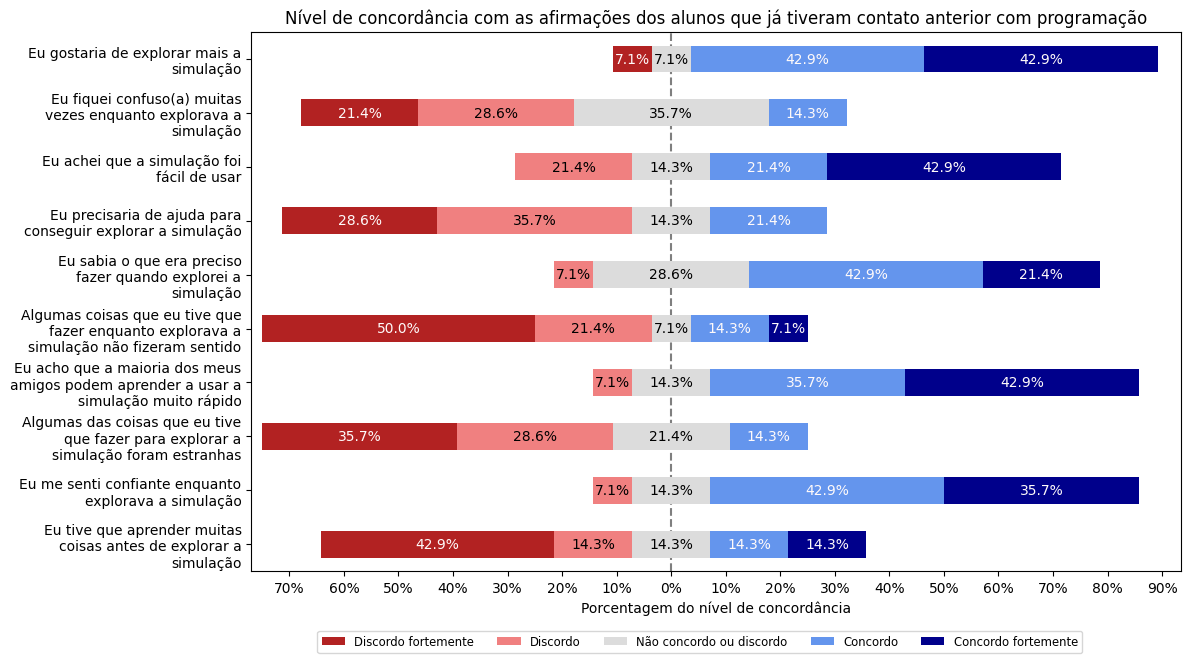
\includegraphics[scale=0.5]{likert_com_conhecimento.png}
    \caption{Porcentagem do nível de concordância com as afirmações dos alunos que já tiveram contato anterior com programação.}
    \label{figure:likert_sim}
\end{figure}

\begin{figure}[h!]
    \centering
    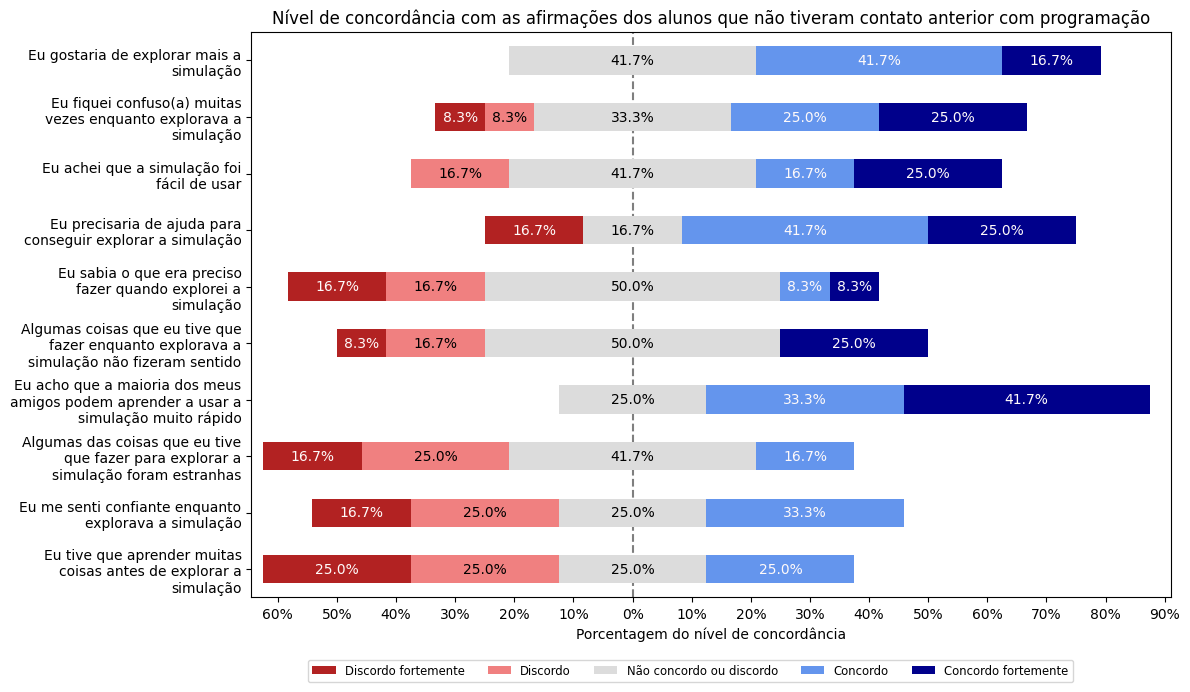
\includegraphics[scale=0.5]{likert_sem_conhecimento.png}
    \caption{Porcentagem do nível de concordância com as afirmações dos alunos que não tiveram contato anterior com programação.}
    \label{figure:likert_nao}
\end{figure}


Já na Figura \ref{figure:likert_nao}, podemos observar as respostas dos alunos que não tiveram contato anterior com programação. Dentre eles, mais da metade (58,4\%) respondeu que gostaria de explorar mais a simulação, porém um grande número (41,7\%) não concordou nem discordou da afirmação. Ainda, 50\% dos alunos desse grupo relatou que ficou confuso muitas vezes enquanto explorava o MVP e 33,3\% não concordou nem discordou disso. A maioria (66,7\%) também achou que precisaria de ajuda para usar a simulação e apenas 16,6\% sabia o que era preciso fazer quando usou a ferramenta. Neste último caso, 50\% não concordou nem discordou da afirmação. De forma contraditória, 41,7\% acharam que a ferramenta foi fácil de usar e apenas 16,7\% discordaram. Ademais, metade dos alunos não concordaram nem discordaram de que algumas coisas que tiveram que fazer não fizeram sentido, e apenas 16,7\% acharam que algumas coisas foram estranhas, enquanto 41,7\% não concordaram nem discordaram. Apesar das respostas anteriores, a maioria dos usuários (72\%) acredita que seus amigos poderiam aprender a usar a simulação muito rápido e apenas 25\% acha que teve que aprender muitas coisas antes de explorá-la. Por fim, 33,3\% das crianças relataram que se sentiram confiantes ao explorar o MVP enquanto 41,7\% discordaram.


Ademais, a Figura \ref{figure:radar_medias} apresenta a média dos níveis de concordância com cada afirmativa dos dois grupos de alunos.

\begin{figure}[h!]
    \centering
    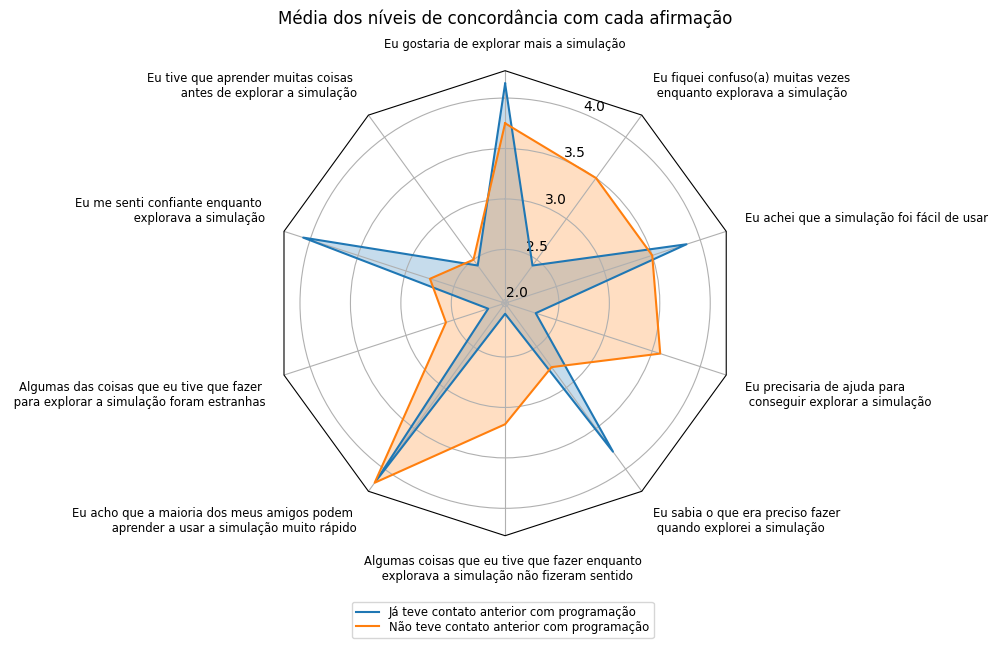
\includegraphics[scale=0.62]{radar_medias.png}
    \caption{Média dos níveis de concordância com cada afirmação dos alunos que já tiveram contato anterior com programação e dos que não tiveram. Cada raio do gráfico representa a média para uma afirmação do formulário.}
    \label{figure:radar_medias}
\end{figure}

Podemos observar que as afirmações do formulário SUS apresentam duas conotações contrárias, tendo algumas delas um sentimento positivo em relação a ferramenta avaliada e outras um sentimento negativo. No questionário, as questões estão intercaladas, de forma que a primeira apresenta um sentimento positivo, a segunda apresenta um sentimento negativo, e assim por diante. Assim, analisando as respostas dos alunos que já tinham um contato prévio com programação, podemos notar que elas estão dentro do esperado, ou seja, em média, os estudantes concordam com as afirmações de caráter positivo e discordam daquelas de caráter negativo. Isso indica que o MPV projetado demonstrou potencial para a continuação ou complementação do aprendizado dos conceitos de lógica de programação das crianças.

Em relação às respostas dos alunos que não tinham contato prévio com programação, observamos algumas inconsistências entre os níveis de concordância com as afirmações de caráter positivo e negativo. Encontramos muitas respostas concordando com afirmações complementares de conotações contrárias. Além disso, em pelo menos metade das afirmações, grande parte dos estudantes permaneceu neutro, optando por não concordar ou discordar, o que não aconteceu com o grupo anterior. Porém, apesar de obtermos muitas respostas concordantes com as afirmações com sentimento negativo em relação ao MVP, a maioria dos estudantes concordou que gostaria de explorar mais a simulação e que seus amigos poderiam aprender a usá-la muito rápido, mostrando o potencial da ferramenta. A partir dessas respostas, verificamos a necessidade de melhorar a forma de introduzir os conceitos de lógica de programação para aqueles que nunca tiveram contato com Computação.

Ademais, calculamos as pontuações SUS, na escala de 0 a 100, para as respostas dos dois grupos de alunos. Para os alunos que já tiveram contato anterior com programação, obtivemos uma média de \textit{score} de 71,6, indicando uma boa usabilidade para o MVP, segundo \citet{bangor2009determining}. Para aqueles que não tinham contato anterior com Computação, a média de pontuação calculada foi de 53,9, o que demonstra usabilidade razoável para a ferramenta de acordo com os autores.

\begin{table}[h!]
\centering
\begin{tabular}{c|c|c|}
\cline{2-3}
                                     & \textbf{\begin{tabular}[c]{@{}c@{}}Já tiveram contato\\ anterior com programação\end{tabular}} & \textbf{\begin{tabular}[c]{@{}c@{}}Não tiveram contato\\ anterior com programação\end{tabular}} \\ \cline{2-3} 
                                     & 82,5                                                                                           & 55                                                                                              \\ \cline{2-3} 
                                     & 75                                                                                             & 50                                                                                              \\ \cline{2-3} 
                                     & 100                                                                                            & 47,5                                                                                            \\ \cline{2-3} 
                                     & 65                                                                                             & 47,5                                                                                            \\ \cline{2-3} 
                                     & 75                                                                                             & 65                                                                                              \\ \cline{2-3} 
                                     & 77,5                                                                                           & 30                                                                                              \\ \cline{2-3} 
                                     & 65                                                                                             & 87,5                                                                                            \\ \cline{2-3} 
                                     & 67,5                                                                                           & 50                                                                                              \\ \cline{2-3} 
                                     & 60                                                                                             & 57,5                                                                                            \\ \cline{2-3} 
                                     & 62,5                                                                                           & 40                                                                                              \\ \cline{2-3} 
                                     & 72,5                                                                                           & 50                                                                                              \\ \cline{2-3} 
                                     & 37,5                                                                                           & 67,5                                                                                            \\ \cline{2-3} 
                                     & 97,5                                                                                           & -                                                                                               \\ \cline{2-3} 
                                     & 65                                                                                             & -                                                                                               \\ \hline
\multicolumn{1}{|c|}{\textbf{média}} & 71,6                                                                                           & 53,9                                                                                            \\ \hline
\end{tabular}
\caption{Pontuação SUS calculada para cada aluno, com as médias para alunos que já tiveram contato anterior com programação e para os que não tiveram.}
\label{table:sus_score}
\end{table}

\subsection**{Opiniões e sugestões sobre a simulação}

Em relação as questões dissertativas sobre opiniões e sugestões da simulação, apresentadas ao final do formulário de usabilidade, quando questionado o que mais gostaram na ferramenta, no geral, as crianças relataram que gostaram da experiência. Dividimos as respostas em quatro categorias baseadas nos temas que se destacaram no \textit{feedback}: recursos específicos, interatividade, experiência de aprendizado e experiência geral. A Figura \ref{figure:livre_1} apresenta os relatos dos estudantes divididos nessas categorias.

\begin{figure}[h!]
    \centering
    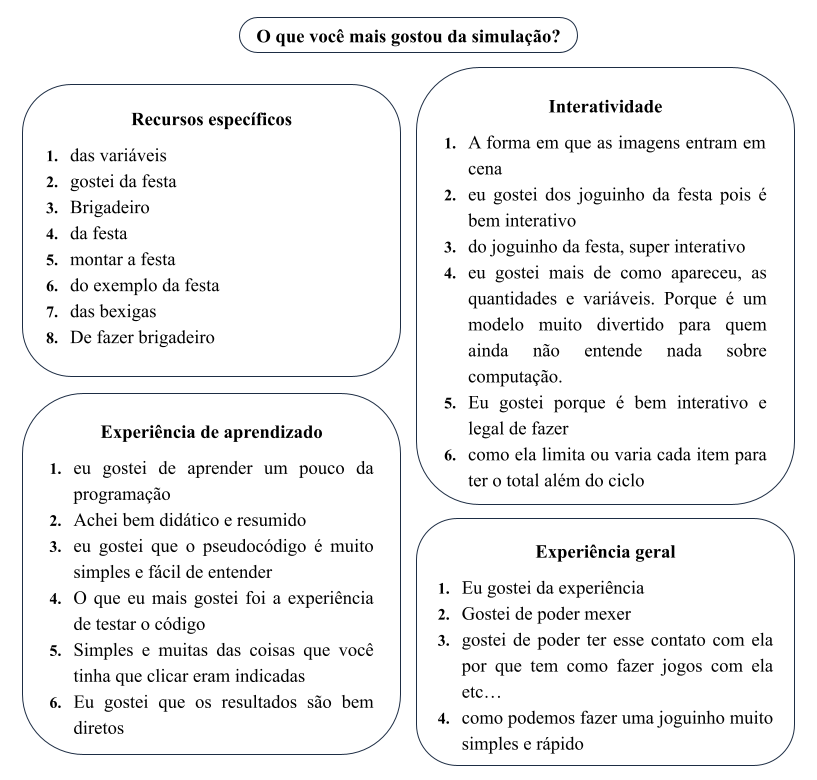
\includegraphics[scale=0.5]{formulario_livre_1.png}
    \caption{Respostas dos alunos em relação à pergunta livre \enquote{O que você mais gostou da simulação?}, divididas em categorias.}
    \label{figure:livre_1}
\end{figure}

Assim, dentre o que as crianças mais gostaram, muitos relataram recursos específicos, como preparar um determinado item para a festa. Além disso, algumas respostas ressaltaram a interatividade da simulação como ponto positivo, como os elementos visuais se apresentavam. Outros relatos destacaram boas experiências de aprendizado e no geral, descrevendo o MVP como didático, simples e direto.

Sobre o que menos gostaram da simulação, observamos outras quatro categorias em que se encaixavam os temas de respostas dos alunos: experiência positiva geral, confusão ou dificuldade, \textit{design} ou problemas de interação, e conteúdo ou tarefas. A Figura \ref{figure:livre_2} apresenta os relatos dos estudantes divididos nessas categorias. Muitos alunos não observaram pontos negativos na experiência geral com a simulação. Por outro lado, muitos encontraram dificuldades e relataram que ficaram confusos, principalmente com o pseudocódigo, ou que acharam complicado. Algumas crianças também apontaram alguns problemas de \textit{design} ou interatividade no MVP e limitações nas possíveis tarefas.

\begin{figure}[h!]
    \centering
    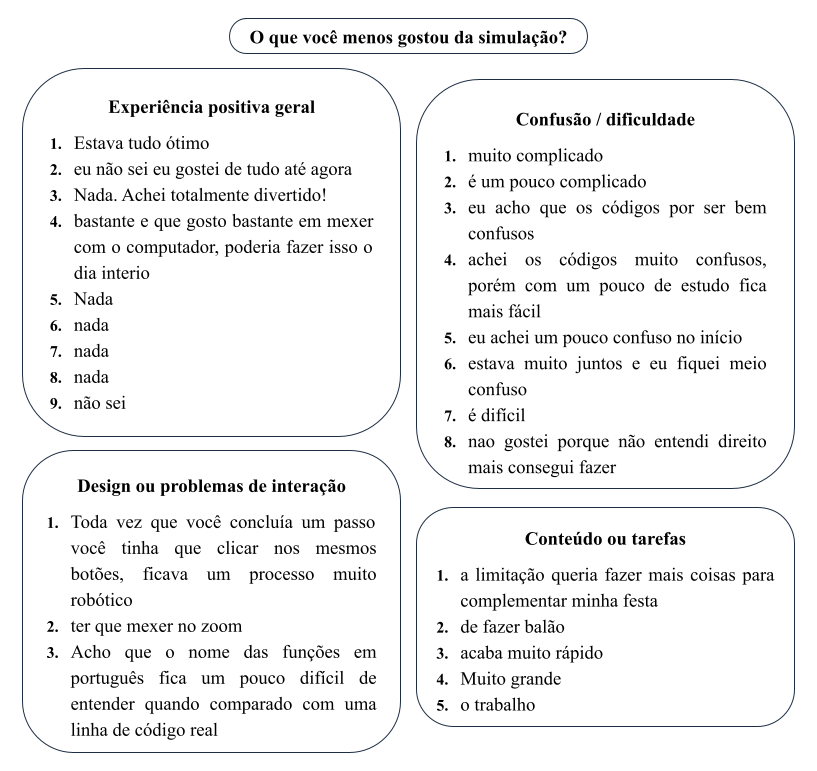
\includegraphics[scale=0.5]{formulario_livre_2.png}
    \caption{Respostas dos alunos em relação à pergunta livre \enquote{O que você menos gostou da simulação?}, divididas em categorias.}
    \label{figure:livre_2}
\end{figure}

Por fim, recebemos comentários referentes a apreciação e divertimento em relação à experiência com a simulação, e complexidade dela, além de sugestões para organizar os códigos, como mostra a Figura \ref{figure:livre_3}. A partir das opiniões e sugestões recebidas nas três questões livres, podemos também constatar a necessidade de algumas modificações nas interações da simulação, bem como na apresentação do pseudocódigo correspondente para tentar diminuir a complexidade encontrada por alguns e melhorar a usabilidade da ferramenta.

\begin{figure}[h!]
    \centering
    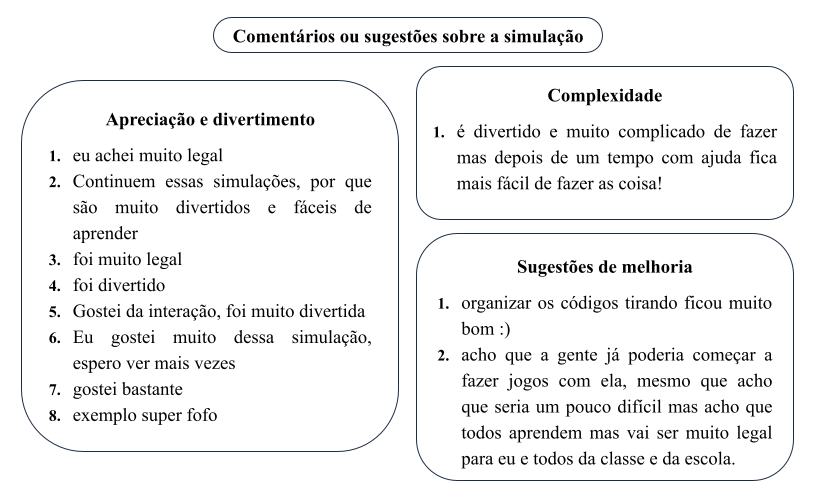
\includegraphics[scale=0.5]{formulario_livre_3.png}
    \caption{Respostas dos alunos em relação à pergunta livre sobre comentários e sugestões da simulação, divididas em categorias.}
    \label{figure:livre_3}
\end{figure}

\section{Atividade de aprendizado}

O questionário com a atividades de aprendizado foi respondido por 13 alunos após o preenchimento do formulário anterior. Das 13 respostas, 6 foram de alunos que nunca tiveram contanto com programação e 7 de alunos que já tiveram. Ainda, dos 6 alunos, apenas 3 responderam a segunda parte da atividade, referente à simulação \enquote{Guardando os Brinquedos}. Para analisar as respostas, separamos os resultados entre os dois grupos de estudantes.

\subsection{Perguntas sobre a simulação \enquote{Planejando a Festa}}

A Figura \ref{figure:pies_festa} apresenta as respostas dos alunos às questões relacionadas à simulação \enquote{Planejando a Festa}. A pergunta 1 tinha como resposta o conceito de \enquote*{condicional}. Considerando os alunos que já tinham um contato anterior com programação, 42,9\% acertou esta questão, outros 42,9\% escolheram o conceito de \enquote*{variáveis} e 14,3\%, o de \enquote*{saída}. Dentre os demais alunos, que nunca tiveram contato com Computação, 33,3\% escolheu a resposta certa, enquanto 50\% respondeu \enquote*{variáveis} e 14,3\% escolheu \enquote*{saída}. Podemos observar que houve confusão entre o conceito de \enquote*{condicional} e o de \enquote*{variáveis} e \enquote*{saída} pelos dois grupos de estudantes. Entretanto, no trecho de pseudocódigo apresentado nessa questão (Figura \ref{figure:atividade_festa_1}) temos a repetição dos dois conceitos que foram confundidos como resposta na execução dentro dos condicionais, o que poderia explicar o engano.

No caso da questão 2, que tinha como resposta \enquote*{variáveis}, observamos que houve uma confusão entre esse conceito e o de \enquote*{entrada}, que também foi notada no geral. Nessa pergunta, 57,1\% dos alunos com conhecimento prévio de Computação acertaram a resposta enquanto 42,9\% escolheram \enquote*{entrada}. Dos alunos que não tinham conhecimento prévio, tivemos um número menor de acertos (33,3\%) e o restante também respondeu \enquote*{entrada}.

\begin{figure}[h!]
    \centering
    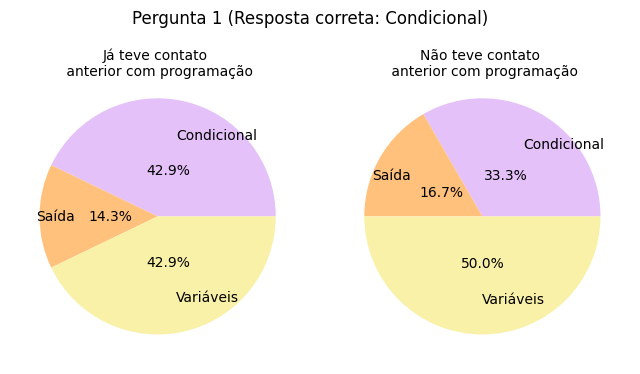
\includegraphics[scale=0.46]{pie_festa_p1.png}
    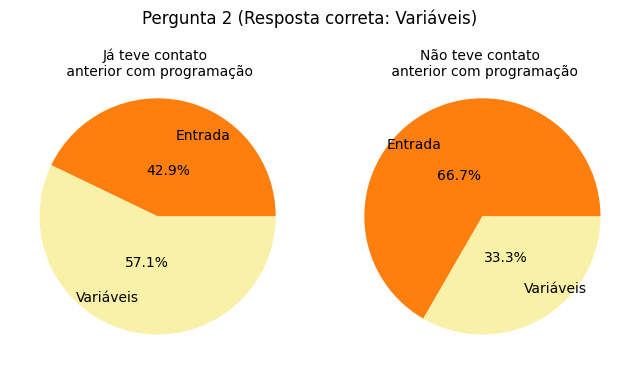
\includegraphics[scale=0.46]{pie_festa_p2.png}
    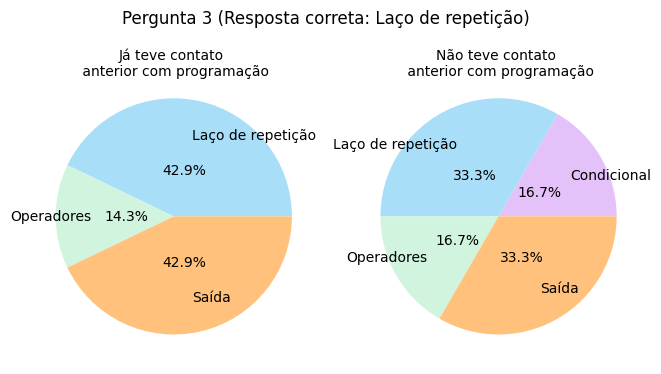
\includegraphics[scale=0.46]{pie_festa_p3.png}
    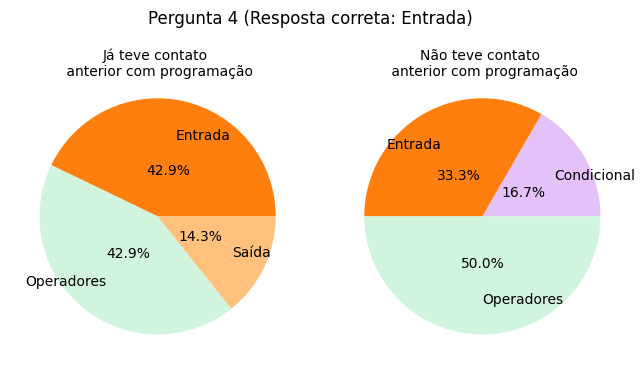
\includegraphics[scale=0.45]{pie_festa_p4.png}
    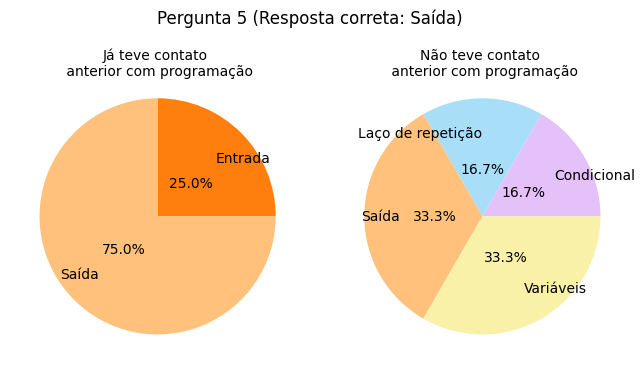
\includegraphics[scale=0.45]{pie_festa_p5.png}
    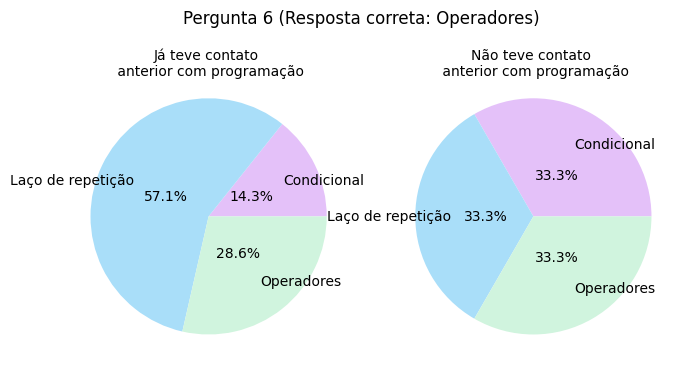
\includegraphics[scale=0.44]{pie_festa_p6.png}
    
\includegraphics[scale=0.35]{pie_legend.png}
    \caption{Porcentagens das respostas dos alunos às perguntas da atividade de aprendizado relacionada à simulação \enquote{Planejando a Festa}. Para cada pergunta, apresentamos as respostas dos alunos que já tiveram contanto anterior com Computação à esquerda e as dos que não tiveram à direita.}
    \label{figure:pies_festa}
\end{figure}

Já na pergunta 3, a resposta correta era \enquote*{laço de repetição}. Das crianças que tiveram contato anterior com programação, 42,9\% acertaram a questão e os demais responderam \enquote*{saída} (42,9\%) e \enquote*{operadores} (14,3\%). Já entre os alunos que não tiveram contato anterior com Computação, 33,3\% escolheram a resposta correta, enquanto 33,3\% escolheram o conceito de \enquote*{saída}, 16,7\% de \enquote*{operadores} e outros 16,7\% de \enquote*{condicional}. Nesta questão tivemos muitas respostas divergentes, assim como na pergunta 1. O trecho de pseudocódigo apresentado nela (Figura \ref{figure:atividade_festa_3}) trazia além do laço de repetição, o conceito de operadores representado na condição do laço e dentro da execução dele, o que poderia justificar a escolha desta resposta por alguns alunos. Além disso, acreditamos também que a ação de preparar um item, a qual ocorre dentro do laço, possa ter sido confundida com o conceito de \enquote*{saída}, respondido por outros. Entretanto, a escolha do conceito de \enquote*{condicional} por alguns estudantes indica a falta de compreensão deles.

Nas três última questões, também observamos que não houve entendimento da maior parte dos alunos em relação aos conceitos de lógica de programação. A quarta pergunta do questionário tinha como resposta o conceito de \enquote*{entrada}. Nela, observamos que 42,9\% dos alunos com conhecimento em programação acertaram a questão. Outras resposta foram \enquote*{operadores} (42,9\%) e \enquote*{saída} (14,3\%). Dos alunos sem conhecimento prévio em Computação, 33,3\% escolheram a resposta certa, enquanto 50\% responderam \enquote*{operadores} e 16,7\% \enquote*{condicional}. 

Na pergunta 5, que tinha como resposta o conceito de \enquote*{saída}, a maioria das crianças com conhecimento anterior de programação acertou (75\%) e apenas 25\% confundiram com de \enquote*{entrada}. Dos alunos sem conhecimento anterior 33,3\% responderam corretamente e os demais alunos responderam \enquote*{variáveis} (33,3\%), \enquote*{condicional} (16,7\%) e \enquote*{laço de repetição} (16,7\%).

Por fim, na questão 6 a resposta correta era \enquote*{operadores} e poucos alunos acertaram o conceito apresentado. Entre as crianças que já tiveram contato com Computação, apenas 28,6\% acertou a resposta. A maior parte das respostas foi \enquote*{laço de repetição} (57,1\%) e os demais responderam \enquote*{condicional} (14,3\%). Entre os estudantes que nunca tiveram contato com programação, as respostas foram igualmente escolhidas entre \enquote*{operadores}, \enquote*{laço de repetição} e \enquote*{condicional}.

\subsection{Perguntas sobre a simulação \enquote{Guardando os Brinquedos}}

A Figura \ref{figure:pies_brinquedos} apresenta as respostas dos alunos às questões relacionadas à simulação \enquote{Guardando os Brinquedos}, com a qual não houve interação. As crianças apenas visualizaram a imagem de um estado da simulação e do pseudocódigo completo. No geral, podemos observar que as crianças com conhecimento prévio em programação fizeram mais confusões em relação aos conceitos de programação abordados do que os demais alunos.

A primeira pergunta tinha como resposta \enquote*{condicional} e, dos alunos que já tiveram contato com Computação, 85,7\% acertaram, enquanto 14,3\% responderam \enquote*{variáveis}. Entre aqueles que não conheciam programação, 66,7\% escolheram a resposta correta e 33,3\% responderam o conceito de \enquote*{saída}. Nesta questão, novamente, observamos que o trecho de pseudocódigo apresentado (Figura \ref{figure:atividade_brinquedos_1}) continha também os demais conceitos escolhidos como resposta por alguns estudantes, o que poderia explicar a confusão.

\begin{figure}[h!]
    \centering
    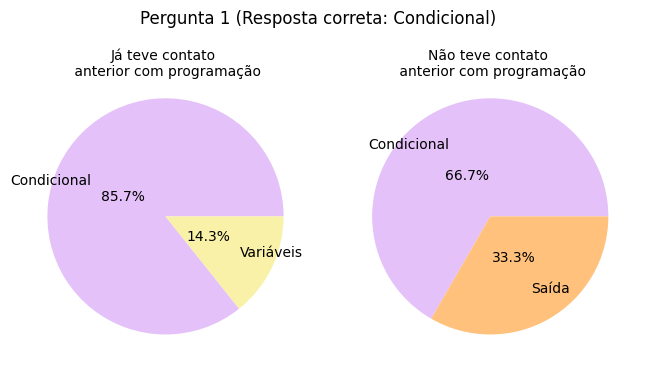
\includegraphics[scale=0.45]{pie_brinquedos_p1.png}
    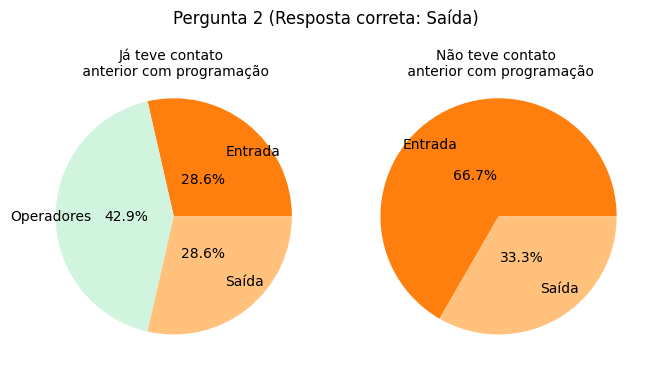
\includegraphics[scale=0.45]{pie_brinquedos_p2.png}
    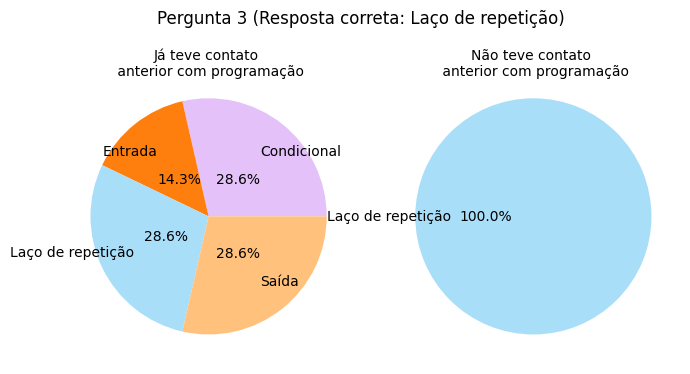
\includegraphics[scale=0.43]{pie_brinquedos_p3.png}
    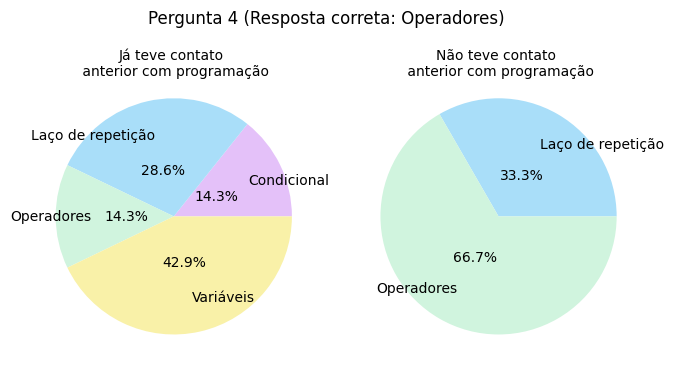
\includegraphics[scale=0.44]{pie_brinquedos_p4.png}
    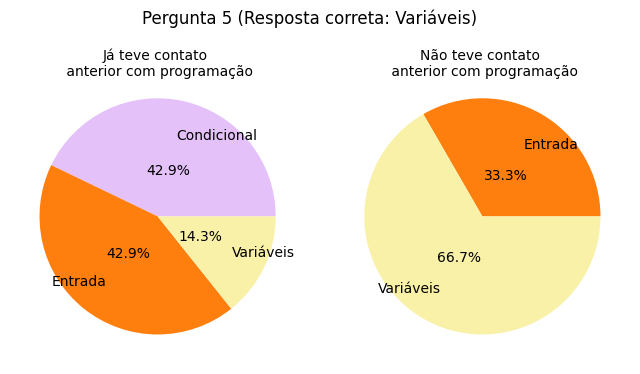
\includegraphics[scale=0.45]{pie_brinquedos_p5.png}
    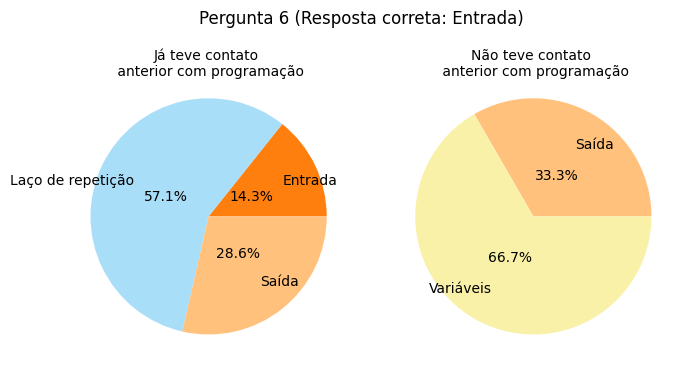
\includegraphics[scale=0.44]{pie_brinquedos_p6.png}
    
\includegraphics[scale=0.35]{pie_legend.png}
    \caption{Porcentagens das respostas dos alunos às perguntas da atividade de aprendizado relacionada à simulação \enquote{Guardando os Brinquedos}. Para cada pergunta, apresentamos as respostas dos alunos que já tiveram contanto anterior com Computação à esquerda e as dos que não tiveram à direita.}
    \label{figure:pies_brinquedos}
\end{figure}

Já na questão 2, cuja resposta era \enquote*{saída}, houve problemas de compreensão dos conceitos por parte da maioria das crianças. Entre aquelas que já conheciam programação, apenas 28,6\% acertaram a resposta, enquanto 42,9\% escolheram \enquote*{operadores} e 28,6\% escolheram \enquote*{entrada}. Entre os alunos que não conheciam Computação, 33,3\% deles acertaram e 66,7\% escolheram \enquote*{entrada}.

Na pergunta 3, em que a resposta correta era \enquote*{laço de repetição}, as duas crianças que não tinham contato anterior com Computação e responderam a questão, acertaram. Dentre os demais alunos, que já tiveram contato, 28,6\% acertaram a resposta e o restante escolheu os conceitos de \enquote*{saída} (28,6\%), \enquote*{condicional} (28,6\%) e \enquote*{entrada} (14,3\%). Porém, ressaltamos que todos os conceitos citados estavam presentes no trecho de pseudocódigo apresentado para eles na pergunta (Figura \ref{figure:atividade_brinquedos_3}).

Já a pergunta 4 tinha como resposta o conceito de \enquote*{operadores}. Entre os alunos que conheciam Computação, apenas 14,3\% acertaram a questão, e a maioria (42,9\%) respondeu \enquote*{variáveis}. Outros escolheram \enquote*{laço de repetição} (28,6\%) e \enquote*{condicional} (14,3\%). Entre os alunos que não tinham conhecimento, a maioria (66,7\%) acertou a resposta e 33,3\% respondeu \enquote*{laço de repetição}. Nessa questão, o trecho de pseudocódigo apresentado (Figura \ref{figure:atividade_brinquedos_4}) trazia uma operação sendo atribuída a uma variável. Assim, a confusão com o conceito de \enquote*{variáveis} pode ter ocorrido por isso. Entretanto, a escolha das demais respostas mostrou, novamente, a falta de compreensão dos conceitos de programação por parte das crianças.

Ademais, nas duas últimas questões, também observamos que não houve entendimento dos alunos em relação aos conceitos. Na questão 5, em que a resposta era \enquote*{variáveis}, dos alunos que tiveram contato anterior com programação, apenas 14,3\% acertaram, enquanto 42,9\% responderam \enquote*{entrada} e 42,9\% responderam \enquote*{condicional}. Dos estudantes sem conhecimento prévio, 66,7\% respondeu \enquote*{variáveis} e 33,3\% \enquote*{entrada}.

Finalmente, na pergunta 6, a resposta correta era \enquote*{entrada}. Entre as crianças que conheciam Computação, apenas 14,3\% acertou a resposta, 57,1\% apontaram de forma errada o conceito de \enquote*{laço de repetição} e 28,6\% o de \enquote*{saída}. Dentre os três alunos que nunca tiveram contato com programação, nenhum acertou essa questão, 66,7\% deles confundiu o conceito com o de \enquote*{variáveis} e 33,3\% escolheu \enquote*{saída}.

A partir desses resultados, observamos que o uso das simulações não cumpriu a finalidade de ensinar os conceitos de lógica de programação para as crianças. Entretanto, como observado, algumas confusões dos conceitos de programação pelos alunos podem ter sido causadas pela formulação das questões da atividade de aprendizado. A presença de muitos conceitos, que inclusive se repetiam, nos trechos de pseudocódigo apresentados em algumas questões pode ter gerado ambiguidade nas respostas. Ainda assim, aqueles conceitos que foram apresentados de forma isolada, como o trecho de \enquote*{variáveis}, não poderia ter sido confundido com o de \enquote*{condicional}, por exemplo, sendo completamente desrelacionado. Isso também indica a falta  de entendimento do conteúdo apresentado.

Ademais, notamos que os alunos sem conhecimento prévio em programação tiveram um maior número de acertos nas questões relacionadas à simulação \enquote{Guardando os Brinquedos}, com a qual eles não interagiram. Isso poderia sugerir a necessidade de alterações e melhorias nas interações implementadas na simulação \enquote{Planejando a Festa}. Por fim, acreditamos que, no geral, os resultados indicaram a necessidade de diversas reformulações para o MVP, implicando em uma nova iteração nos ciclos de \textit{design} e engenharia de DSR.

